\documentclass{oxblue-beamer}

\usepackage{multicol}
\setlength\columnsep{20pt}

\title{Solving the 15-Puzzle Problem \\ with A* and IDS Algorithms}
\subtitle{CS Elec 1 Midterm Project}
\author[Mape, Lucero, Latoza, \& Eclarinal]{
    Rixdon Niño Mape                \inst{1} \and
    Jerwin Glen Lucero              \inst{1} \and \\
    Hannah Isabel Latoza            \inst{1} \and
    Alexandra Nicole Eclarinal      \inst{1}
}
\institute[BUCS]{
    \inst{1}
    Bicol University,                                       \\
    College of Science,                                     \\
    Computer Science and Information Technology Department  \\
}
\date{\today}

\begin{document}

\begin{frame}
\titlepage
\end{frame}

\section{Overview}

\begin{frame}{Overview}
\begin{itemize}
    \item What's the problem? \textbf{15-puzzle}
    \item What's the proposed solution? \textbf{A* search and IDS algorithms}
    \item What's the main approach in solving the problem?
    \begin{enumerate}
        \item Read the initial board state from the user.
        \item Check if the puzzle is solvable.
        \item Create the initial node.
        \item Perform a search algorithm and measure the running time.
        \item Print the solution, runtime, expanded nodes, and the moves.
    \end{enumerate}
\end{itemize}
\end{frame}

\begin{frame}[fragile]{Sample Output}
\begin{verbatim}
Enter the initial board state (0-15, space-separated):
1 5 2 3 6 0 7 11 4 12 14 10 9 8 13 15
The board is solvable.
Running Time: 0.000000 seconds
Nodes expanded: 35
Moves in the solution: 16
Solution: START L D D R U L D R R U R U L L U L
\end{verbatim}
\end{frame}

\begin{frame}{Results}
\begin{itemize}
    \item For all test cases, \textbf{A* search was faster than IDS} since it expanded fewer nodes while discovering a similar solution.
    \item For each implementation of both algorithms, the \textbf{worst test case is not solved} because of failed memory allocation for successor nodes.
\end{itemize}
\end{frame}

\begin{frame}{Results (cont.)}
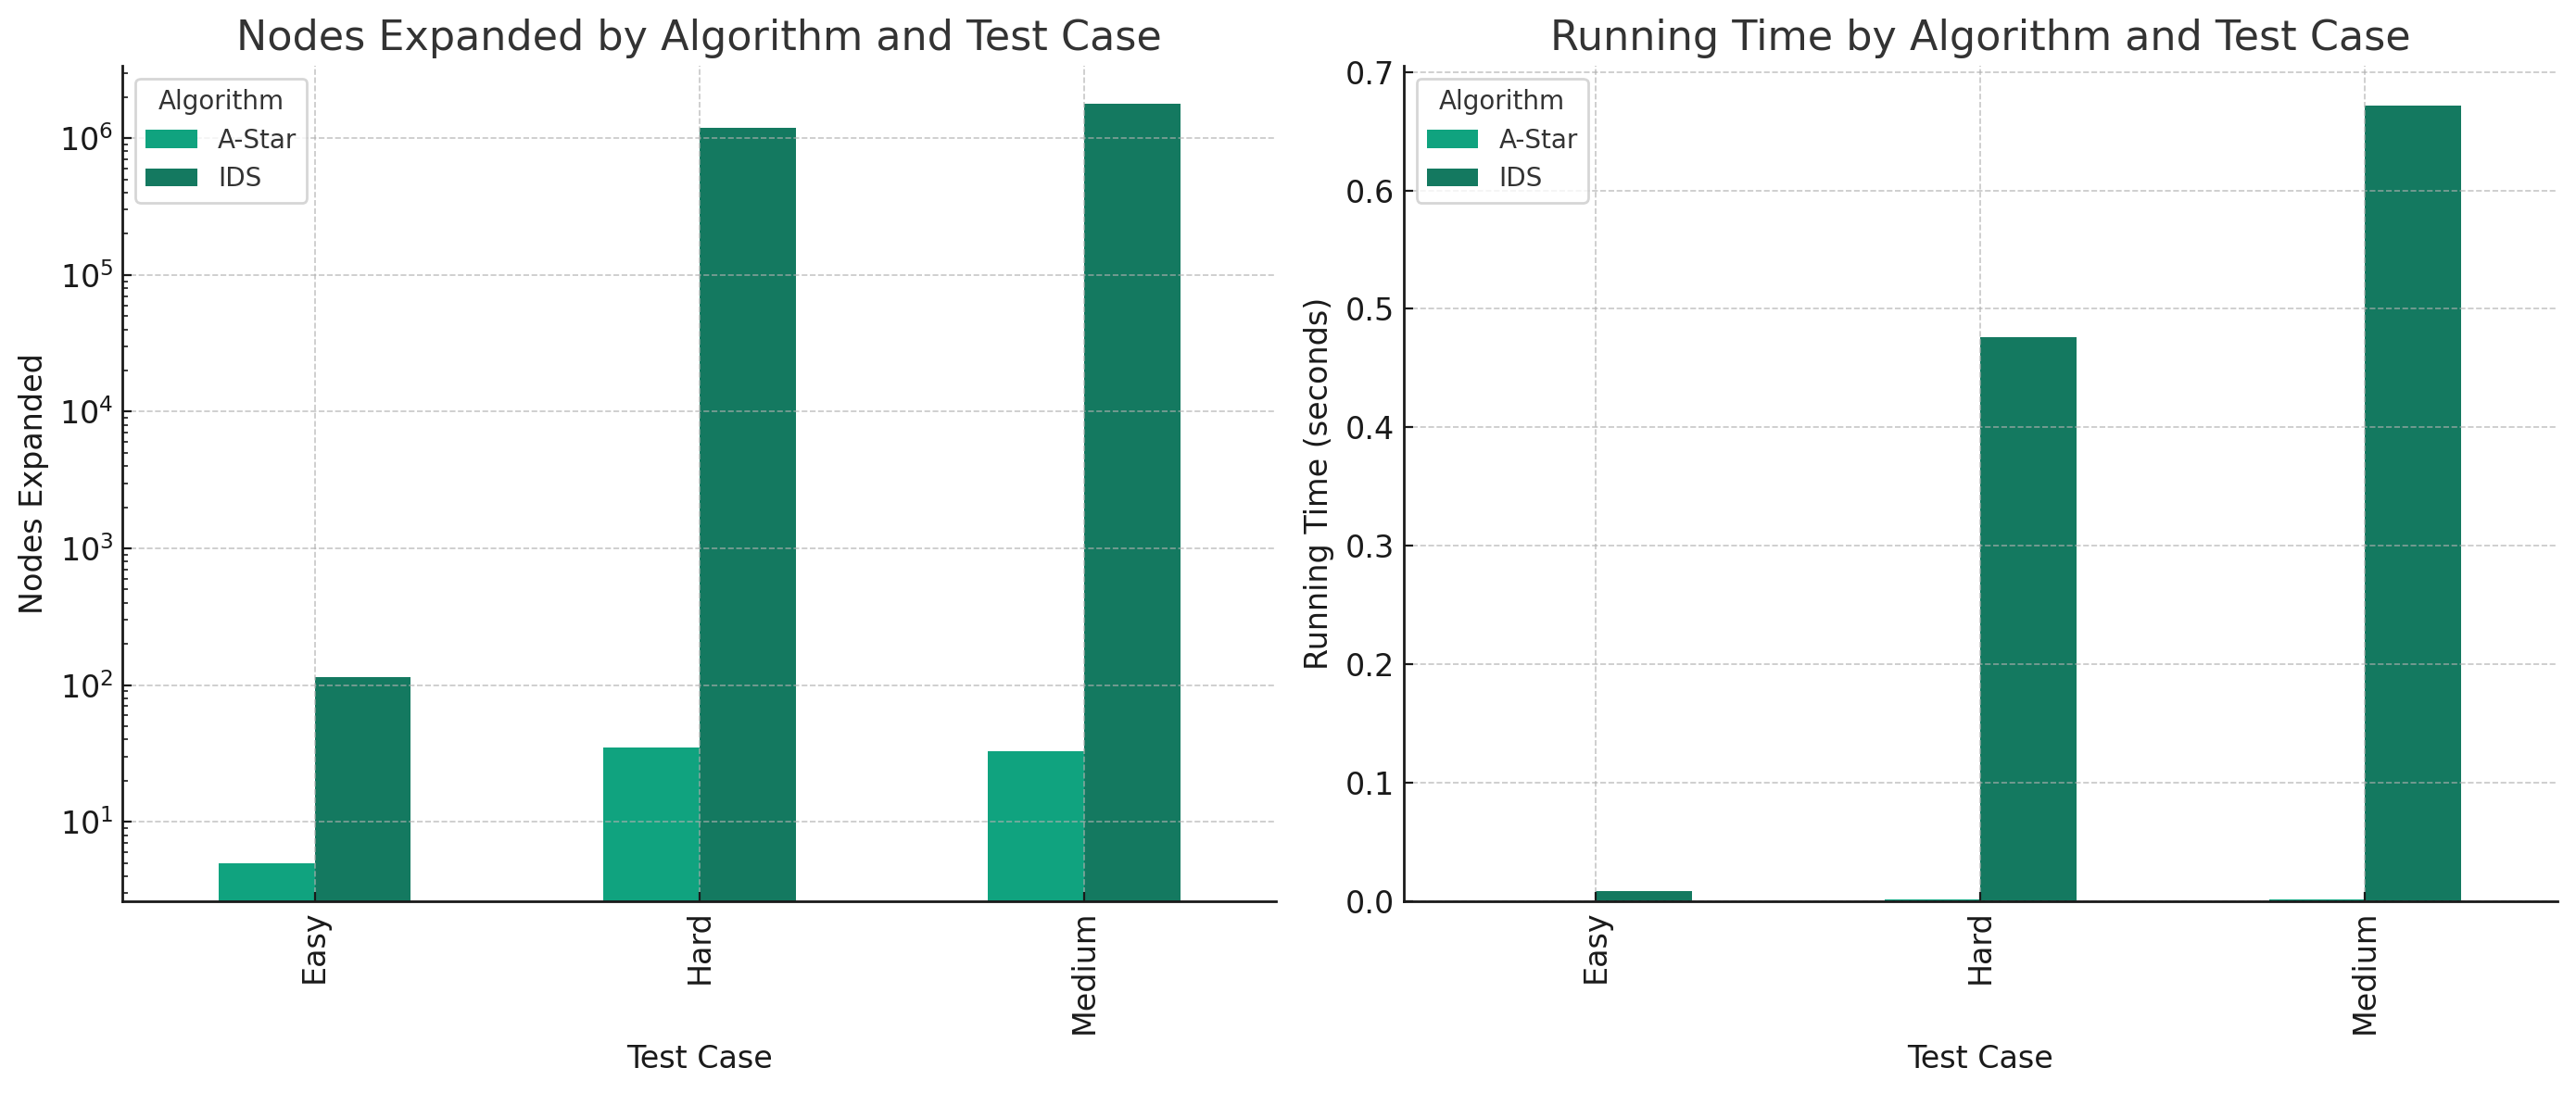
\includegraphics[width=\textwidth]{assets/results.png}
\end{frame}

\section{Shared Constants, Data Structures, and Functions}

\begin{frame}{Constants}
\begin{itemize}
    \item \mintinline{c}|BOARD_SIZE 16|
    \item \mintinline{c}|BOARD_ROW_SIZE 4|
    \item \mintinline{c}|BLANK_TILE 0|
    \item \mintinline{c}|POSSIBLE_MOVES 4|
    \item \mintinline{c}|LOAD_FACTOR 0.75|
    \item \mintinline{c}|INITIAL_CAPACITY 1000000|
    \item \mintinline{c}|CAPACITY_MULTIPLIER 2|
\end{itemize}
\end{frame}

\begin{frame}[fragile]{Data Structures}
\begin{multicols}{2}
\begin{minted}{c}
typedef enum Move {
    INITIAL = 0,
    UP = -4,
    DOWN = 4,
    LEFT = -1,
    RIGHT = 1
} Move;
\end{minted}
\columnbreak
\begin{minted}{c}
typedef struct Node {
    struct Node* parent;
    int board[BOARD_SIZE];
    size_t priority;
    Move move;
    size_t g;
    size_t h;
    size_t f;
} Node;
\end{minted}
\end{multicols}
\end{frame}

\begin{frame}{Utility Functions}
\begin{itemize}
    \item \mintinline{c}|Node* create_initial_node(int board[BOARD_SIZE])|
    \item \mintinline{c}|Node* create_child_node(Node* current, Move move)|
    \item \mintinline{c}|bool is_goal(int board[BOARD_SIZE])|
    \item \mintinline{c}|size_t get_blank_tile_index(int board[BOARD_SIZE])|
    \item \mintinline{c}|size_t get_inversion(int board[BOARD_SIZE])|
    \item \mintinline{c}|bool is_solvable(int board[BOARD_SIZE])|
    \item \mintinline{c}|bool is_valid_move(int board[BOARD_SIZE], Move move)|
    \item \mintinline{c}|void apply_move(int board[BOARD_SIZE], Move move)|
    \item \mintinline{c}|void print_moves(Node* node)|
\end{itemize}
\end{frame}

\section{Implementation of A* Search Algorithm}

\begin{frame}[fragile]{Data Structures}
\begin{multicols}{2}
\begin{minted}{c}
typedef struct HashTable {
    int** arr;
    size_t size;
    size_t capacity;
} HashTable;
\end{minted}
\columnbreak
\begin{minted}{c}
typedef struct PriorityQueue {
    Node** nodes;
    size_t size;
    size_t capacity;
} PriorityQueue;
\end{minted}
\end{multicols}
\end{frame}

\begin{frame}{Hash Table Functions}
\begin{itemize}
    \item \mintinline{c}|HashTable* create_hash_table(size_t capacity)|
    \item \mintinline{c}|size_t hash_value(int board[BOARD_SIZE], size_t size)|
    \item \mintinline{c}|void resize_hash_table(HashTable* ht)|
    \item \mintinline{c}|void insert_to_hash_table(HashTable* ht, int board[BOARD_SIZE])|
    \item \mintinline{c}|bool is_in_hash_table(HashTable* ht, int board[BOARD_SIZE])|
    \item \mintinline{c}|void delete_hash_table(HashTable* ht)|
\end{itemize}
\end{frame}

\begin{frame}{Priority Queue Functions}
\begin{itemize}
    \item \mintinline{c}|PriorityQueue* create_priority_queue(size_t capacity)|
    \item \mintinline{c}|void heapify_up(Node** nodes, size_t index)|
    \item \mintinline{c}|void heapify_down(Node** nodes, size_t size, size_t index)|
    \item \mintinline{c}|void resize_priority_queue(PriorityQueue* pq)|
    \item \mintinline{c}|void push_to_priority_queue(PriorityQueue* pq, Node* node)|
    \item \mintinline{c}|Node* pop_from_priority_queue(PriorityQueue* pq)|
    \item \mintinline{c}|Node* search_priority_queue(PriorityQueue* pq, int board[BOARD_SIZE])|
    \item \mintinline{c}|void delete_priority_queue(PriorityQueue* pq)|
\end{itemize}
\end{frame}

\begin{frame}[fragile]{A* Search Algorithm Functions}
\begin{minted}{c}
Node* a_star_search(PriorityQueue* open, HashTable* closed, Node* initial) {
    push_to_priority_queue(open, initial);
    while (open->size > 0) {
        Node* current = pop_from_priority_queue(open);
        if (is_goal(current->board)) return current;
        insert_to_hash_table(closed, current->board);
        Move moves[POSSIBLE_MOVES] = {UP, DOWN, LEFT, RIGHT};
        for (size_t i = 0; i < POSSIBLE_MOVES; ++i) {
            if (!is_valid_move(current->board, moves[i])) continue;
            Node* child = create_child_node(current, moves[i]);
            if (is_in_hash_table(closed, child->board)) continue;
            Node* open_node = search_priority_queue(open, child->board);
\end{minted}
\end{frame}

\begin{frame}[fragile]{A* Search Algorithm Functions (cont.)}
\begin{minted}[firstnumber=13]{c}
            if (open_node == NULL) {
                push_to_priority_queue(open, child);
            } else if (child->f < open_node->f) {
                open_node->parent = child->parent;
                open_node->g = child->g;
                open_node->h = child->h;
                open_node->f = child->f;
                open_node->move = child->move;
                heapify_up(open->nodes, open_node->priority);
            }
        }
    }
    return NULL;
}
\end{minted}
\end{frame}

\begin{frame}[fragile]{A* Search Algorithm Functions (cont.)}
\begin{minted}{c}
int manhattan_distance(int board[BOARD_SIZE]) {
    int total_distance = 0;
    for (size_t i = 0; i < BOARD_SIZE; ++i) {
        int tile = board[i];
        if (tile == BLANK_TILE) continue;
        int current_row = i / BOARD_ROW_SIZE;
        int current_col = i % BOARD_ROW_SIZE;
        int target_row = tile / BOARD_ROW_SIZE;
        int target_col = tile % BOARD_ROW_SIZE;
        int distance =
            abs(current_row - target_row) + abs(current_col - target_col);
        total_distance += distance;
    }
    return total_distance;
}
\end{minted}
\end{frame}

\section{Implementation of Iterative-Deepening Search Algorithm}

\begin{frame}[fragile]{Data Structure}
\begin{minted}{c}
typedef struct Stack {
    Node** nodes;
    size_t size;
    size_t capacity;
} Stack;
\end{minted}
\end{frame}

\begin{frame}{Stack Functions}
\begin{itemize}
    \item \mintinline{c}|Stack* create_stack(size_t capacity)|
    \item \mintinline{c}|void resize_stack(Stack* stack)|
    \item \mintinline{c}|void push_to_stack(Stack* stack, Node* node)|
    \item \mintinline{c}|Node* pop_from_stack(Stack* stack)|
    \item \mintinline{c}|Node* search_stack(Stack* stack, int board[BOARD_SIZE])|
    \item \mintinline{c}|void delete_stack(Stack* stack)|
\end{itemize}
\end{frame}

\begin{frame}[fragile]{IDS Algorithm Functions}
\begin{minted}{c}
Node* iterative_deepening_search(Node* initial) {
  int depth = 0;
  while (1) {
    Stack* open = create_stack(INITIAL_CAPACITY);
    Node* result = depth_limited_search(open, initial, depth);
    if (result != NULL) return result;
    depth++;
  }
}
\end{minted}
\end{frame}

\begin{frame}[fragile]{IDS Algorithm Functions (cont.)}
\begin{minted}{c}
Node* depth_limited_search(Stack* open, Node* node, int limit) {
    push_to_stack(open, node);
    while (open->size > 0) {
        Node* current = pop_from_stack(open);
        expanded_nodes_counter++;
        if (is_goal(current->board)) return current;
        if (current->depth >= limit || is_cycle(current)) continue;
        Move moves[POSSIBLE_MOVES] = {UP, DOWN, LEFT, RIGHT};
        for (size_t i = 0; i < POSSIBLE_MOVES; ++i) {
            if (!is_valid_move(current->board, moves[i])) continue;
            Node* child = create_child_node(current, moves[i]);
            push_to_stack(open, child);
        }
    }
    return NULL;
}
\end{minted}
\end{frame}

\begin{frame}
\centering \Large
Thank you for your attention!
\end{frame}

\end{document}
